\clearpage\pagenumbering{arabic}
\chapter{Overview}\label{Overview}
Coast is a platform for developing and deploying World Wide Web
applications. It provides an extensible framework, reusable
components, and a configuration mechanism that is used to create web
applications. For deployment, it provides an efficient and scaleable
server and additional flexible communication infrastructure.\\
\\
In this chapter we give an overview of the environment and challenges
posed by server programming and web application programming.

\section{WWW Environment}
The World Wide Web bases on the Hypertext Transfer Protocol (HTTP). It
is an application-level protocol for distributed, collaborative,
hypermedia information systems. It is a generic, stateless, protocol
which can be used for many tasks beyond its use for hypertext, such as
name servers and distributed object management systems, through
extension of its request methods, error codes and headers. A feature
of HTTP is the typing and negotiation of data representation, allowing
systems to be built independently of the data being transferred.

\begin{figure}[hbt]
  \centering
  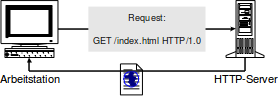
\includegraphics[width=0.6\hsize]{chap01/request_reply_protocol}
  \caption{Request reply protocol.}
  \label{fig:request_reply_protocol}
\end{figure}

An important type of content transferred is HTML. It is the lingua
franca for publishing hypertext on the World Wide Web. It is a
non-proprietary format based upon SGML, and can be created and
processed by a wide range of tools, from simple plain text editors -
you type it in from scratch- to sophisticated WYSIWYG authoring tools.
HTML uses tags such as <h1> and </h1> to structure text into headings,
paragraphs, lists, hypertext links etc.

\section{Web Applications}
Very soon people started to publish not only static files but also dynamically
generated content with several extension technologies (CGI\footnote{CGI: Common
Gateway Interface, standard way of extending web server functionality with
dynamic behavior.}, ISAPI\footnote{ISAPI: Internet Server API, API definition
for inprocess extensions of web servers}, NSAPI\footnote{NSAP: Netscape Server
API, Netscapes flavour of extension API}). WebApplications proved as effective
information and functionality deployment vehicle, tying together existing IS
Worlds with a universal UI tool, the Web-browser. But as the Web evolved from
its origins as a simple delivery mechanism — suitable for small files and simple
applications — to a platform for complex applications, Web servers and the
stateless HTTP proved very limiting. New robust, scalable architectures and a
new class of servers to support a high-volume, distributed, and heterogeneous
application environment, were required.\\
\\
To overcome the limitations of HTTP based page serving a WebApplication Server
has to implement additional features.

\subsection{Enabling web access means integration}
Implementing WebApplications means accessing data sources and legacy
applications, since it is neither possible nor useful to re-implement all
existing database systems and applications at once to enable web access.
Enabling web services mostly requires integration of several databases or
existing systems. The mix of services a WebApplication consists of or their
implementation can change very fast and often. A vast range of technologies
exist to access the functionality of existing systems. Needless to say all have
bugs and problems now and then.\\
\\
Essentially two problems exists:

\begin{itemize}
  \item Knowing the details of the system level API and using it correctly.
  \item Finding and correcting problems in case of failures
\end{itemize}

A programmer should not have to care about the details of system level
integration.\\
\\
It should be possible to integrate and manipulate backend systems
without impact on the logic part of the application on a syntactic level.

\subsection{Session Management}
HTTP is a stateless protocol, every information needed to produce a reply is
contained in the request. Implementing a WebApplication this is either not
feasible or inconvenient for the user. To build sophisticated and stable
interactions into web applications we need to keep state. Saving all state in
the request implies overhead and is limited by most browsers and intermediate
proxy-servers. Loosing the state, e.g. because of size limitations, produces
unexpected results. Although WebServers have already defined authentication and
authorization schemas based on Access Control Lists (ACL) or Lightweight
Directory Access Protocol (LDAP), this is mostly too coarse grained or
inflexible for WebApplications. Calculating the user’s authentication and
authorization information on every request is inefficient and puts unnecessary
load on machines. Storing authentication and authorization information between
requests in session store, makes them more efficient and enables better
security, since authentication credentials need not be included in every
request. Sometimes there is also a need to load a lot of data to initialize the
application context on a per user basis. It is faster and more efficient, to do
it once and keep it than to do it on every request. Session information keeps
the state needed to operate the WebApplication in meaningful ways on a per user
basis. Session information has also to be released some when. Since no strict
interaction pattern can be enforced on the web this is best handled by a timeout
mechanism. Using a session, after it is freed, e.g. by using a bookmark, needs
to establish the same session’s state as when the bookmark information was
generated. Reestablishing lost information can be used to automatically enforce
re-authentication rules into secure parts of a WebApplication.

\subsection{Role based access control}
Navigation usually depends on the credentials (e.g. authentication and
authorization) of a user. Navigation paths are grouped into categories (e.g.
public, customer, administration etc.). Using a specific category we like the
user to assume a role into the system, e.g. he uses the system as a guest. This
means he has the access rights a guest has. If access to pages a guest can
access is not restricted, everybody can access those pages and we do not even
need to care about the authentication of the user. As soon as the user wants to
access a restricted area we need to authenticate and authorize the user. This
can be done in any way you like and if successful, the user assumes the new role
needed to visit the restricted area. Depending on the web applications type, the
same user can assume several roles.\\
\\
The access control takes place on two levels:
\begin{itemize}
  \item Role level checks if the session has the correct role with regard to the
  service requested.
  \item Intra role level checks if the session has the right to access this
  service assuming the role level is correct. This allows for fine granular service autorization schemes.
\end{itemize}
Services are only executed if both of those checks succeed. In the failure case
appropriate action takes place, be it a request for re-authentication or sending
back an error message instead of a normal service reply.

\subsection{Dynamic content expansion}
Web applications are based on serving HTML pages. Instead of serving static
content or simple dynamic content (like time of day or number of accesses etc)
those pages are highly dynamic and changing. Most web application servers have
some sort of dynamic page rendering using HTML templates and a macro expansion
mechanism. The rendering of a page takes place in several steps. First of all
the overall template has to be evaluated, then all the dynamic content macros
are expanded. Execution of the macros accesses data that is provided by backend
systems. What if those systems fail to deliver the data as expected? Ideally it
is possible to separate layout of an application from dynamically generated
content. And it is even possible to change layout and structure of the whole
application on the state of some data provided. So if backend systems fail we
can respond with a completely different page as when they are up and running.

\section{COAST Concepts}
COAST has a tool set to implement a wide range of applications, but it is
geared toward implementation of TCP based request-reply servers implementing a
web application. This kind of server is on one hand an efficient Web server that
serves static page content like images and help pages and on the other hand an
application that generates HTML output dynamically using backend datasources
available. In the following sections we shed light on the concepts implemented
in the COAST environment.

\subsection{General Server issues}
This section describes the challenges posed by implementing server software.
Apart from functional requirements a server has always to strive for fullfilling
technical requirements like high availability, fast response time, high
throughput and ease of administration. Ideally a server never crashes, never
leaks and is able to keep a certain level of response time at peak loads.

\subsubsection{Servers and Request processing}
A server is a running process providing a set of services. It is known by a DNS
name (implying an IP-address) and a well known port. Clients requesting service
connect to the server and establish a TCP connection. Over this connection data
is sent and received. A server should not be blocked when request processing is
in progress. There exists two basic approaches to achieve this goal. Several
processes are spawned and act as servers (Multiprocessing). This solution is
stable but produces overhead in the case that information between the processes
has to be shared. The other solution spawns threads (Multithreading) in one
process, which is dangerous in the case of errors, but more efficient with
regard to information sharing. COAST uses multithreading in one process.

\subsubsection{Services and Service Dispatching}
A request is always associated with a service. A service groups requests by any
criteria useful for the purpose of the application (e.g. all local files
publicly accessible, all requests getting their input from database xy etc.).
Services read input and send replies. However to find out which service to use
we already have to read some of the input supplied. We call this service
dispatching. It is done by a specialised component that selects the service.
Service dispatching can be done by any attributes suitable present in the
request (e.g. Port and Address, Source Address or URI Prefix).

\subsubsection{Programming in a MT-Server}
Programming in a multi threaded server allows for efficient sharing of data.
Simply assign a value to a variable seen by more than one thread and it is
usable by all, which have access to it. But this is only half of the story. On
the other hand you have to make sure that under no circumstances shared values
are accessed unprotected, if they are changed by any side. And when you start
locking code to achieve this, all the nasty things called deadlock, live-lock
and starvation, can show up and threaten the quality of the server.
Multi-threading is difficult and error prone to programm. The code has to be
correct in a concurrent world. Therefore an important goal of the architecture
of COAST is to relief the application programmer from the MT-burden as far
possible. A lot of shared objects have read only data. Every request handled has
a context object that handles access to read write stores. The context object is
a local variable of the executing thread so it needs no locking. Essentially
only session information is shared and read/write. For this reason all accesses
to session information and the management of sessions have to be carefully
locked. But any extension, which does not follow the predefined path, has to
consider concurrency aspects carefully.

\subsection{Web application issues}
Web applications refine and add to the requirements we have for a server
application. The protocol used is HTTP therefore a Web application lives in a
request reply world. A web application can be seen as sequence of pages visited
by a user. Each page defines some follow up pages with links. There are fast
entry points in the form of bookmarks, and forward and backward chains in the
form of back and forward buttons in the browser. At each point a user is allowed
to visit some follow up pages based on his authentication credentials. With this
prerequisite we are able to define an enhanced model of request processing.

\subsubsection{Request handling cycle}
A WebApplication service predefines several steps of processing. Each has it‘s
own goal and different objects involved.

\begin{figure}[hbt]
	\centering
\begin{tikzpicture}
  \colorlet{good}{green!75!black}
  \colorlet{bad}{red}
  \colorlet{neutral}{black!60}
  \colorlet{none}{white}
  \draw node[text centered, text width=3cm]{WebApplication Service};
  \begin{scope}[line width=4mm,rotate=270]
    \draw[
    	good,
        decoration={markings, mark=at position 1 with
        {\arrow{stealth}}}, postaction={decorate} ]
        (-123:2cm) arc (-123:-101:2cm);
    \draw[good!60!white] (-36:2cm) arc (-36:-101:2cm);
    \draw[neutral]       (-36:2cm) arc (-36:36:2cm);
    \draw[bad!60!white]  (36:2cm)  arc (36:93:2cm);
    \newcount\mycount
    \foreach \angle in {0,72,...,3599}
    {
      \mycount=\angle\relax
      \divide\mycount by 10\relax
      \draw[black!15,thick] (\the\mycount:18mm) -- (\the\mycount:22mm);
    }
    \draw (0:2.2cm) node[below] {``ok'': 10 (20\%)};
    \draw (165:2.2cm) node[above] {none: 20 (40\%)};
    \draw (-111:2.2cm) node[left] {``very good'': 3 (6\%)};
    \draw (-68:2.2cm) node[left] {``good'': 9 (18\%)};
    \draw (65:2.2cm) node[right] {``bad'': 8 (16\%)};
    \draw (93:2.2cm) node[right] {``very bad'': 0 (0\%)};
  \end{scope}
  \draw[gray] (0,0) circle (2.2cm) circle (1.8cm);
\end{tikzpicture}
	\caption{WebApplication‘s request processing cycle.}
	\label{fig:webservicerequestcycle}
\end{figure}

\begin{figure}[hbt] \centering
\begin{tikzpicture}
  \colorlet{good}{green!75!black}
  \colorlet{bad}{red}
  \colorlet{neutral}{black!60}
  \colorlet{none}{white}
  \draw node[text centered, text width=3cm]{WebApplication Service};
  \begin{scope}[line width=4mm,rotate=90]
    \draw [
    	good!60!white,
    	decoration={markings, mark=at position 1 with { \node [single
        arrow,fill=good!60!white, inner sep=0pt, transform shape] {};}},
        postaction={decorate} ] { (-45:2cm) arc (-45:-90:2cm) };
    \draw [
    	good,
    	decoration={markings, mark=at position 1 with { \node [single
        arrow,fill=good, inner sep=0pt, transform shape] {};}},
        postaction={decorate} ] { (0:2cm) arc (0:-45:2cm) };
    \draw decorate [
    	decoration={text along path,text={this is getting silly}},
        ] { (0:2cm) arc (0:-45:2cm) };
  \end{scope}
\end{tikzpicture}
	\caption{WebApplication‘s request processing cycle.}
	\label{fig:webservicerequestcycleX}
\end{figure}

Analyze request and select the service:
The incoming request is parsed as far as necessary to select the service (e.g.
the HTTP-Header). WebDisplay Web application requests contain four standard
elements of information: session id, role, page and action. They are all used in
the WebDisplay request processing cycle. The Web application service is session
based, therefore we select also the session defined by the request’s sessionid
or create a new one.

\begin{figure}[hbt]
  \centering
  \includegraphics[width=0.5\hsize]{chap01/Acceptor}
  \caption{Acceptor.}
  \label{fig:zipstream}
\end{figure}

\begin{figure}[hbt]
  \centering
  \includegraphics[width=0.9\hsize]{chap01/test}
  \caption{MscGen example.}
  \label{fig:mscgen_example}
\end{figure}
